\clearpage
\section{ Problem 1.}
A code breaker intercepted the encoded message below.\\
45 -35 38 -30 18 -18 35 -30 81 -60 42 -28 75 -55 2 -2 22 -21 15 -10\\[6pt]
Let the inverse of the encoding matrix be $A^{-1} =
\begin{bmatrix}
    w & x \\
    y & z \\
\end{bmatrix}$

\begin{enumerate}[label=(\alph*)]
    \item Given that $[45 \quad -35]A^{-1} = [10\quad 15]$ and $[38\quad -30]A^{-1} = [8\quad 14]$. Write and solve two systems of equations to find $w, x, y,$ and
    $z$.
    \item Decode the message.
\end{enumerate}

\vspace*{1cm}

\textbf{Theory:}\\[6pt]
This problem involves decoding a message that has been encoded using a matrix transformation.\\
To decode the message, we need to multiply each encoded vector by the inverse of A. The inverse of A can be computed using standard methods of matrix inversion, such as Gaussian elimination.\\[6pt]

\textbf{Handwritten solution:}\\[6pt]
We have:
\[
    \begin{bmatrix} 45 & -35 \end{bmatrix}
    \begin{bmatrix} w & x \\y & z \end{bmatrix}
    =
    \begin{bmatrix}
    45w -35y \\
    45x -35z \\
    \end{bmatrix}^T
    =
    \begin{bmatrix} 10 \\ 15 \\ \end{bmatrix}^T
\]

\[
    \begin{bmatrix} 38 & -30 \end{bmatrix}
    \begin{bmatrix} w & x \\y & z \end{bmatrix}
    =
    \begin{bmatrix}
    38w -30y \\
    38x -30z \\
    \end{bmatrix}^T
    =
    \begin{bmatrix} 8 \\ 14 \\ \end{bmatrix}^T
\]

From the above equations, we can write the following system of equations:
\[
\begin{cases}
    45w -35y = 10 \\
    45x -35z = 15 \\
    38w -30y = 8 \\
    38x -30z = 14 \\
\end{cases}
\]

Solve the system of equations using Gaussian Elimination, we get:
\[
\begin{cases}
    w = 1 \\
    x = -2 \\
    y = 1 \\
    z = -3 \\
\end{cases}
\]

Therefore, the inverse of A is:
\[
    A^{-1} =
    \begin{bmatrix}
    1 & -2 \\
    1 & -3 \\
    \end{bmatrix}
\]

After that, we can decode the message by multiplying each encoded vector by the inverse of A.

\vspace*{1cm}

\textbf{Python code:}
\lstinputlisting[language=Python]{code/problem1.py}

\vspace*{0.5cm}

\textbf{Result:}
\begin{figure}[H]
    \centering
    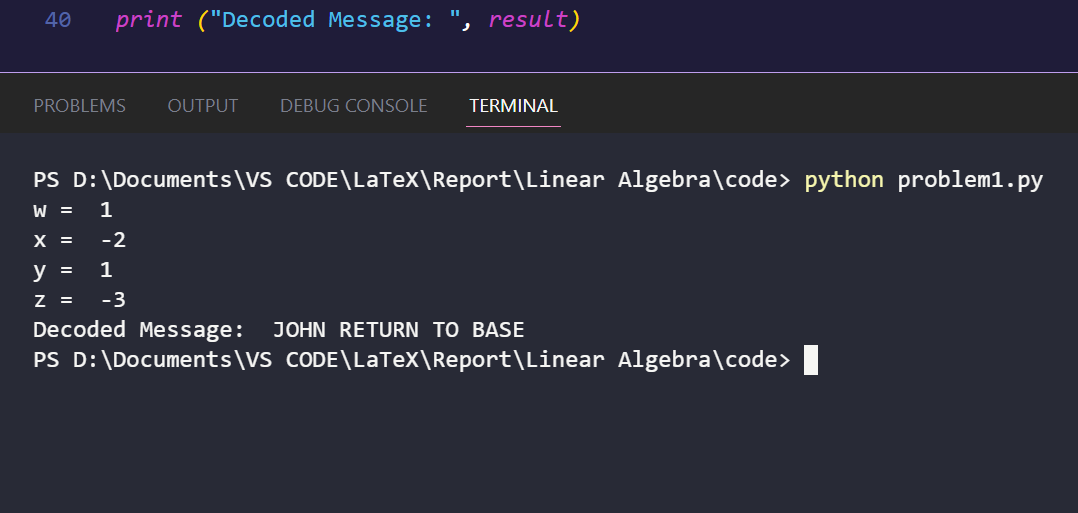
\includegraphics[width=16cm]{graphics/1.png}
    \caption{Console output of problem1.py}
\end{figure}